\documentclass{article}
\usepackage[a4paper,left=3cm, right=3cm, top=2cm, bottom=2cm]{geometry}
\usepackage{amsmath}
\usepackage{graphicx}
\usepackage{caption}
\usepackage{setspace}
\usepackage{xcolor}
\usepackage{titlesec}
\usepackage{amssymb}
\graphicspath{{graph/}}
\title{10.5 Conic Sections}
\date{}
\author{}
\setstretch{1.2} 

% \subsection* 형식 지정 (번호 없음)
\titleformat{name=\section, numberless}
  {\normalfont\large\bfseries\color{blue}}
  {}
  {0pt}
  {}
\geometry{a4paper, margin=1in}

\begin{document}
\maketitle
In this section we give geometric definitions of parabolas, ellipses, and hyperbolas and derive their standard equations. They are called conic sections, or conics, because they result from intersecting a cone with a plane as shown in Figure 1.
\begin{figure}[htbp]
    \centering
    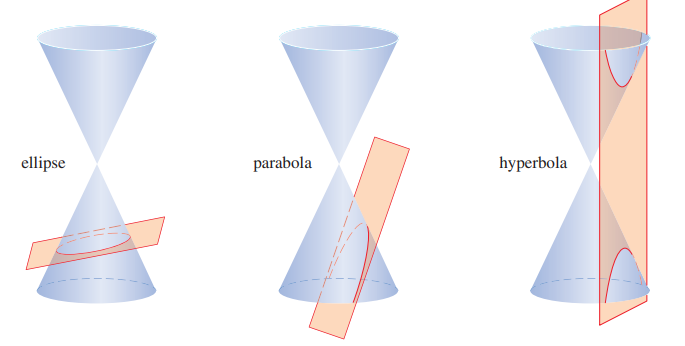
\includegraphics[width=0.6\textwidth]{graph50.png}
\end{figure}


\section*{Parabolas}
Galileo showed that the path of a projectile that is shot into the air at an angle to the ground is a parabola. Parabola shapes have been used in designing automobile headlights, reflection telescopes, and suspension bridges.

A parabola is the set of points in a plane that are equidistant from a fixed point F (called the focus) and a fixed line (called the directrix). The point halfway between the focus and the directrix lies on the parabola; it is called the vertex. The line through the focus perpendicular to the directrix is called the axis of the parabola.
\begin{figure}[htbp]
    \centering
    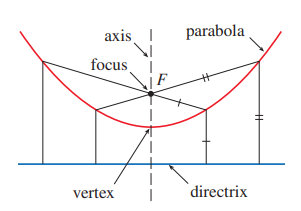
\includegraphics[width=0.3\textwidth]{graph51.png}
    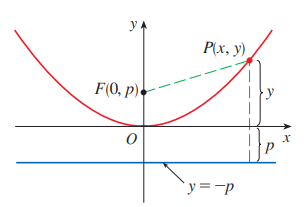
\includegraphics[width=0.3\textwidth]{graph52.png}
\end{figure}
We obtain a particularly simple equation for a parabola if we place its vertex at the origin O and its directrix parallel to the x-axis. If the focus is the point $(0,p)$, then the directrix has the equation $y=-p$. If $P(x,y)$ is any point on the parabola, then the distance from P to the focus is $|PF| = \sqrt{x^2 + (y-p)^2}$ and the distance from P to the directrix is $|y+p|$.

The defining property of a parabola is that these distances are equal:
\[
\sqrt{x^2 + (y-p)^2} = |y+p|
\]
Squaring and simplifying leads to:
\begin{align*}
    x^2 + (y-p)^2 &= (y+p)^2 \\
    x^2 + y^2 - 2py + p^2 &= y^2 + 2py + p^2 \\
    x^2 &= 4py
\end{align*}

\begin{enumerate}
    \item An equation of the parabola with focus $(0,p)$ and directrix $y=-p$ is $x^2 = 4py$. This parabola opens upward if $p > 0$ and downward if $p < 0$.
    \item An equation of the parabola with focus $(p,0)$ and directrix $x=-p$ is $y^2 = 4px$. This parabola opens to the right if $p > 0$ and to the left if $p < 0$.
\end{enumerate}
\begin{figure}[htbp]
    \centering
    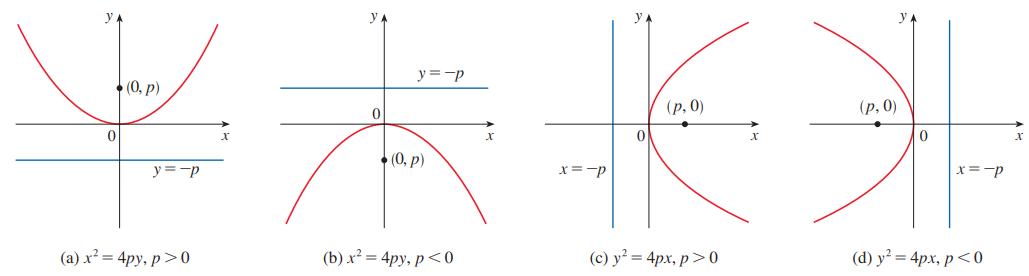
\includegraphics[width=1\textwidth]{graph53.png}
\end{figure}

\subsubsection*{EXAMPLE 1}
Find the focus and directrix of the parabola $y^2 + 10x = 0$ and sketch the graph.

\paragraph{Solution:} If we write the equation as $y^2 = -10x$ and compare it with Equation 2, we see that $4p = -10$, so $p = -5/2$. Thus the focus is $(-5/2, 0)$ and the directrix is $x = 5/2$.

\section*{Ellipses}
\begin{figure}[htbp]
    \centering
    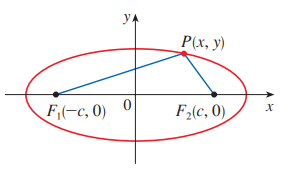
\includegraphics[width=0.35\textwidth]{graph55.png}
\end{figure}
An ellipse is the set of points in a plane the sum of whose distances from two fixed points $F_1$ and $F_2$ is a constant. These two fixed points are called the foci.

To obtain the simplest equation, we place the foci on the x-axis at $(\pm c, 0)$. Let the sum of the distances from a point on the ellipse to the foci be $2a > 0$. Then a point $P(x,y)$ is on the ellipse when $|PF_1| + |PF_2| = 2a$. This leads to the equation:
\[
\frac{x^2}{a^2} + \frac{y^2}{b^2} = 1
\]
where $b^2 = a^2 - c^2$. The points $(\pm a,0)$ are called the vertices.

\paragraph{The ellipse $\frac{x^2}{a^2} + \frac{y^2}{b^2} = 1$} where $a > b > 0$ has foci $(\pm c, 0)$, where $c^2 = a^2 - b^2$, and vertices $(\pm a, 0)$.

\paragraph{The ellipse $\frac{x^2}{b^2} + \frac{y^2}{a^2} = 1$} where $a > b > 0$ has foci $(0, \pm c)$, where $c^2 = a^2 - b^2$, and vertices $(0, \pm a)$.
\begin{figure}[htbp]
    \centering
    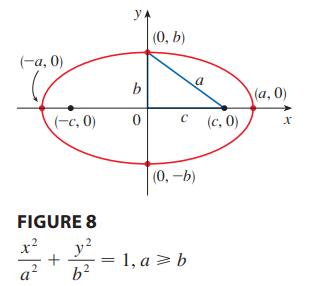
\includegraphics[width=0.3\textwidth]{graph 55.png}
    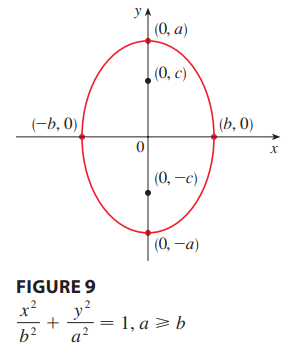
\includegraphics[width=0.3\textwidth]{graph54.png}
\end{figure}
\subsubsection*{EXAMPLE 2}
Sketch the graph of $9x^2 + 16y^2 = 144$ and locate the foci.

\paragraph{Solution:} Divide both sides by 144:
\[
\frac{x^2}{16} + \frac{y^2}{9} = 1
\]
So $a^2 = 16$, $b^2 = 9$, which means $a=4, b=3$. Also, $c^2 = a^2 - b^2 = 16 - 9 = 7$, so $c = \sqrt{7}$. The foci are $(\pm\sqrt{7}, 0)$.

\subsubsection*{EXAMPLE 3}
Find an equation of the ellipse with foci $(0, \pm2)$ and vertices $(0, \pm3)$.

\paragraph{Solution:}
Here $c=2$ and $a=3$. Then $b^2 = a^2 - c^2 = 9 - 4 = 5$. The equation is $\frac{x^2}{5} + \frac{y^2}{9} = 1$, or $9x^2 + 5y^2 = 45$.

\section*{Hyperbolas}
\begin{figure}[htbp]
    \centering
    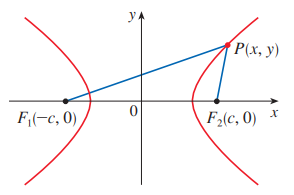
\includegraphics[width=0.3\textwidth]{graph56.png}
\end{figure}
A hyperbola is the set of all points in a plane the difference of whose distances from two fixed points $F_1$ and $F_2$ (the foci) is a constant. With foci on the x-axis at $(\pm c, 0)$, the equation is:
\[
\frac{x^2}{a^2} - \frac{y^2}{b^2} = 1
\]
where $c^2 = a^2 + b^2$. The points $(\pm a,0)$ are the vertices. The asymptotes are $y = \pm(b/a)x$.

\paragraph{The hyperbola $\frac{x^2}{a^2} - \frac{y^2}{b^2} = 1$} has foci $(\pm c, 0)$, vertices $(\pm a, 0)$, and asymptotes $y = \pm(b/a)x$.

\paragraph{The hyperbola $\frac{y^2}{a^2} - \frac{x^2}{b^2} = 1$} has foci $(0, \pm c)$, vertices $(0, \pm a)$, and asymptotes $y = \pm(a/b)x$.
\begin{figure}[htbp]
    \centering
    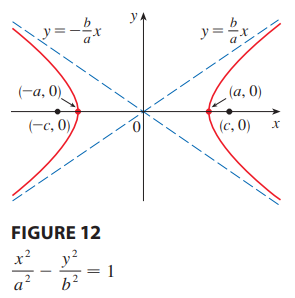
\includegraphics[width=0.3\textwidth]{graph57.png}
    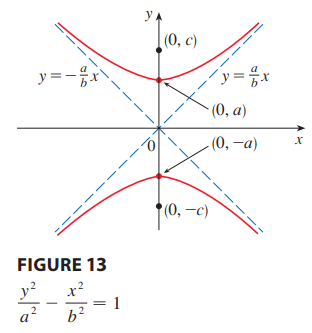
\includegraphics[width=0.3\textwidth]{graph58.png}
\end{figure}
\subsubsection*{EXAMPLE 4}
Find the foci and asymptotes of $9x^2 - 16y^2 = 144$.

\paragraph{Solution:} Divide by 144: $\frac{x^2}{16} - \frac{y^2}{9} = 1$.
So $a=4$, $b=3$. $c^2 = a^2 + b^2 = 16+9=25$, so $c=5$.
Foci: $(\pm5, 0)$. Asymptotes: $y = \pm\frac{3}{4}x$.

\subsubsection*{EXAMPLE 5}
Find the foci and equation of the hyperbola with vertices $(0, \pm1)$ and asymptote $y = 2x$.

\paragraph{Solution:}
From the vertices, $a=1$. From the asymptote, $a/b = 2 \implies 1/b = 2 \implies b = 1/2$.
Then $c^2 = a^2 + b^2 = 1 + 1/4 = 5/4$.
Foci: $(0, \pm\sqrt{5}/2)$. Equation: $y^2 - 4x^2 = 1$.

\section*{Shifted Conics}
We shift conics by replacing $x$ and $y$ with $x-h$ and $y-k$ in the standard equations.

\subsubsection*{EXAMPLE 6}
Find an equation of the ellipse with foci $(2, -2)$, $(4, -2)$ and vertices $(1, -2)$, $(5, -2)$.

\paragraph{Solution:}
The center is the midpoint of the vertices: $(3, -2)$. The distance from the center to a vertex is $a = 2$. The distance from the center to a focus is $c = 1$.
$b^2 = a^2 - c^2 = 4 - 1 = 3$. The equation is:
\[
\frac{(x-3)^2}{4} + \frac{(y+2)^2}{3} = 1
\]

\subsubsection*{EXAMPLE 7}
Sketch the conic $9x^2 - 4y^2 - 72x + 8y + 176 = 0$ and find its foci.

\paragraph{Solution:}
Complete the square:
\begin{align*}
    (9x^2 - 72x) - (4y^2 - 8y) &= -176 \\
    9(x^2 - 8x) - 4(y^2 - 2y) &= -176 \\
    9(x^2 - 8x + 16) - 4(y^2 - 2y + 1) &= -176 + 9(16) - 4(1) \\
    9(x-4)^2 - 4(y-1)^2 &= -176 + 144 - 4 \\
    9(x-4)^2 - 4(y-1)^2 &= -36 \\
    \frac{4(y-1)^2}{36} - \frac{9(x-4)^2}{36} &= 1 \\
    \frac{(y-1)^2}{9} - \frac{(x-4)^2}{4} &= 1
\end{align*}
This is a hyperbola with center $(4,1)$. Here $a^2=9, b^2=4$, so $c^2 = a^2+b^2=13$.
Foci: $(4, 1 \pm \sqrt{13})$. Vertices: $(4, 1 \pm 3)$, which are $(4,4)$ and $(4,-2)$.
Asymptotes: $y-1 = \pm\frac{3}{2}(x-4)$.
\begin{figure}[htbp]
    \centering
    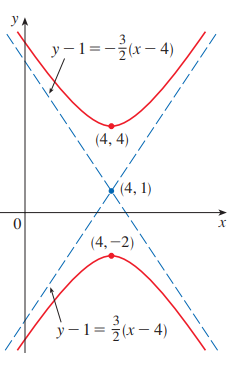
\includegraphics[width=0.3\textwidth]{graph59.png}
\end{figure}
\end{document}
